\documentclass[12pt, titlepage]{article}
\usepackage{graphicx}
\usepackage{anysize}
\usepackage{dsfont}
\usepackage{fullpage}
\usepackage{verbatim}
\usepackage{url}
\usepackage{dsfont}
\usepackage[titletoc]{appendix}
\usepackage{tocloft}
\usepackage{url,amsfonts, amssymb, amsthm,color, enumerate, multicol}
\usepackage{amsmath}
\usepackage{placeins}
\usepackage{titlesec}
\usepackage{csvsimple, longtable, booktabs, makecell,siunitx}

\usepackage{mathtools}

\renewcommand{\thesection}{\Roman{section}} 
\renewcommand{\thesubsection}{\thesection.\Roman{subsection}}

%\titleformat*{\section}{\normalfont\bfseries}

% Ceil and Floor
\DeclarePairedDelimiter{\ceil}{\lceil}{\rceil}
\DeclarePairedDelimiter\floor{\lfloor}{\rfloor}
%\noprintanswers

\setlength{\cftsecnumwidth}{4em}

\begin{document}

\title{\LARGE \textbf{ Benford's Law} \\
	\vspace{2ex}
	\large VE401 Probabilistic Methods in Engineering \\
    Project 1 (Summer 2017)}
\date{June 26, 2017}
\author{\textit{Siddharth Ramesh, Ziwen Lu, Kevin Zheng, Derek Tan, Chengcheng Zhu}}

\maketitle
\pagenumbering{gobble}
\pagebreak
\tableofcontents
\pagebreak
\setcounter{page}{1}
\pagenumbering{arabic}

\section{Abstract}

Benford's law \cite{benford} is an interesting generalization on how the frequency of the leading digits behave in real life. Intuitively, we would think that, with a large dataset, the distribution of the leading digits would be uniform, 1/9 for every digit $\in \{1, 2, 3, 4, 5, 6, 7, 8, 9\}$. However, as seen in practice, this is not always the case. This report will explore Benford's law and its property of scale invariance, a proof written by Roger Pinkham \cite{pinkham}, as well as the shortcomings of Pinkham's proof as expressed in a proof by Theodore Hill \cite{hill}.

\section{Scale Invariance}

Let's first investigate the property of re-scaling; this implies that the distribution of the leading digit cannot be uniform. \\

Let X be a uniformly distributed discrete random variable that corresponds to the first digit, where each digit occurs with probability $\frac{1}{9}$. Assume that, after scaling, then this distribution is independent of re-scaling, meaning that the probability of each digit being a leading digit is still $\frac{1}{9}$. \\

We denote $P[X = m]$ to mean the probability that the first digit is m, where $m \in \{1, 2, 3, 4, 5, 6, 7, 8, 9\}$, and $P_\alpha[X = m]$ to mean the probability that the first digit is m, after rescaling to a nonzero factor $\alpha$. By our assumption, 
\begin{equation*}
P[X = m] = P_\alpha[X = m]. \\ 
\end{equation*}

By observation, if a number starts with 5, 6, 7, 8, 9, then scaling with a factor $\alpha = 2$ will cause the number to begin with 1. This means that
\begin{equation*}
\begin{split}
P_2[X = 1]  \geq P[X = 5 \cap 6 \cap 7 \cap 8 \cap 9] = \frac{5}{9} \neq P[X = 1]\\ 
\end{split}
\end{equation*}
Thus, there is a contradiction between (1) and (2), meaning that the discrete uniformly distributed variable X is not independent of rescaling in all cases. \\

Benford's law is remarkable in that it applies in a wide variety of natural numbers, such as populations, lengths of rivers, mathematical constants, etc. We have analyzed the periodic tables of elements to show this.

\section{Data Visualization}
We will examine Benford's law in practice through a natural data set, such as the Elastic Properties of the Elements \cite{elements}. Below, we have plotted the frequencies of the shear modulus of every element, as well as the frequencies of their leading numbers. A table of the raw data can be found in Appendix A.
Visually, the data in Figure 1 seems to be distributed expontentially, with the elements' shear modulus skewed towards lower values. \\

\begin{figure}
\caption{Frequencies of the Shear Modulus of the Elements in GPa \cite{elements}}
\centering
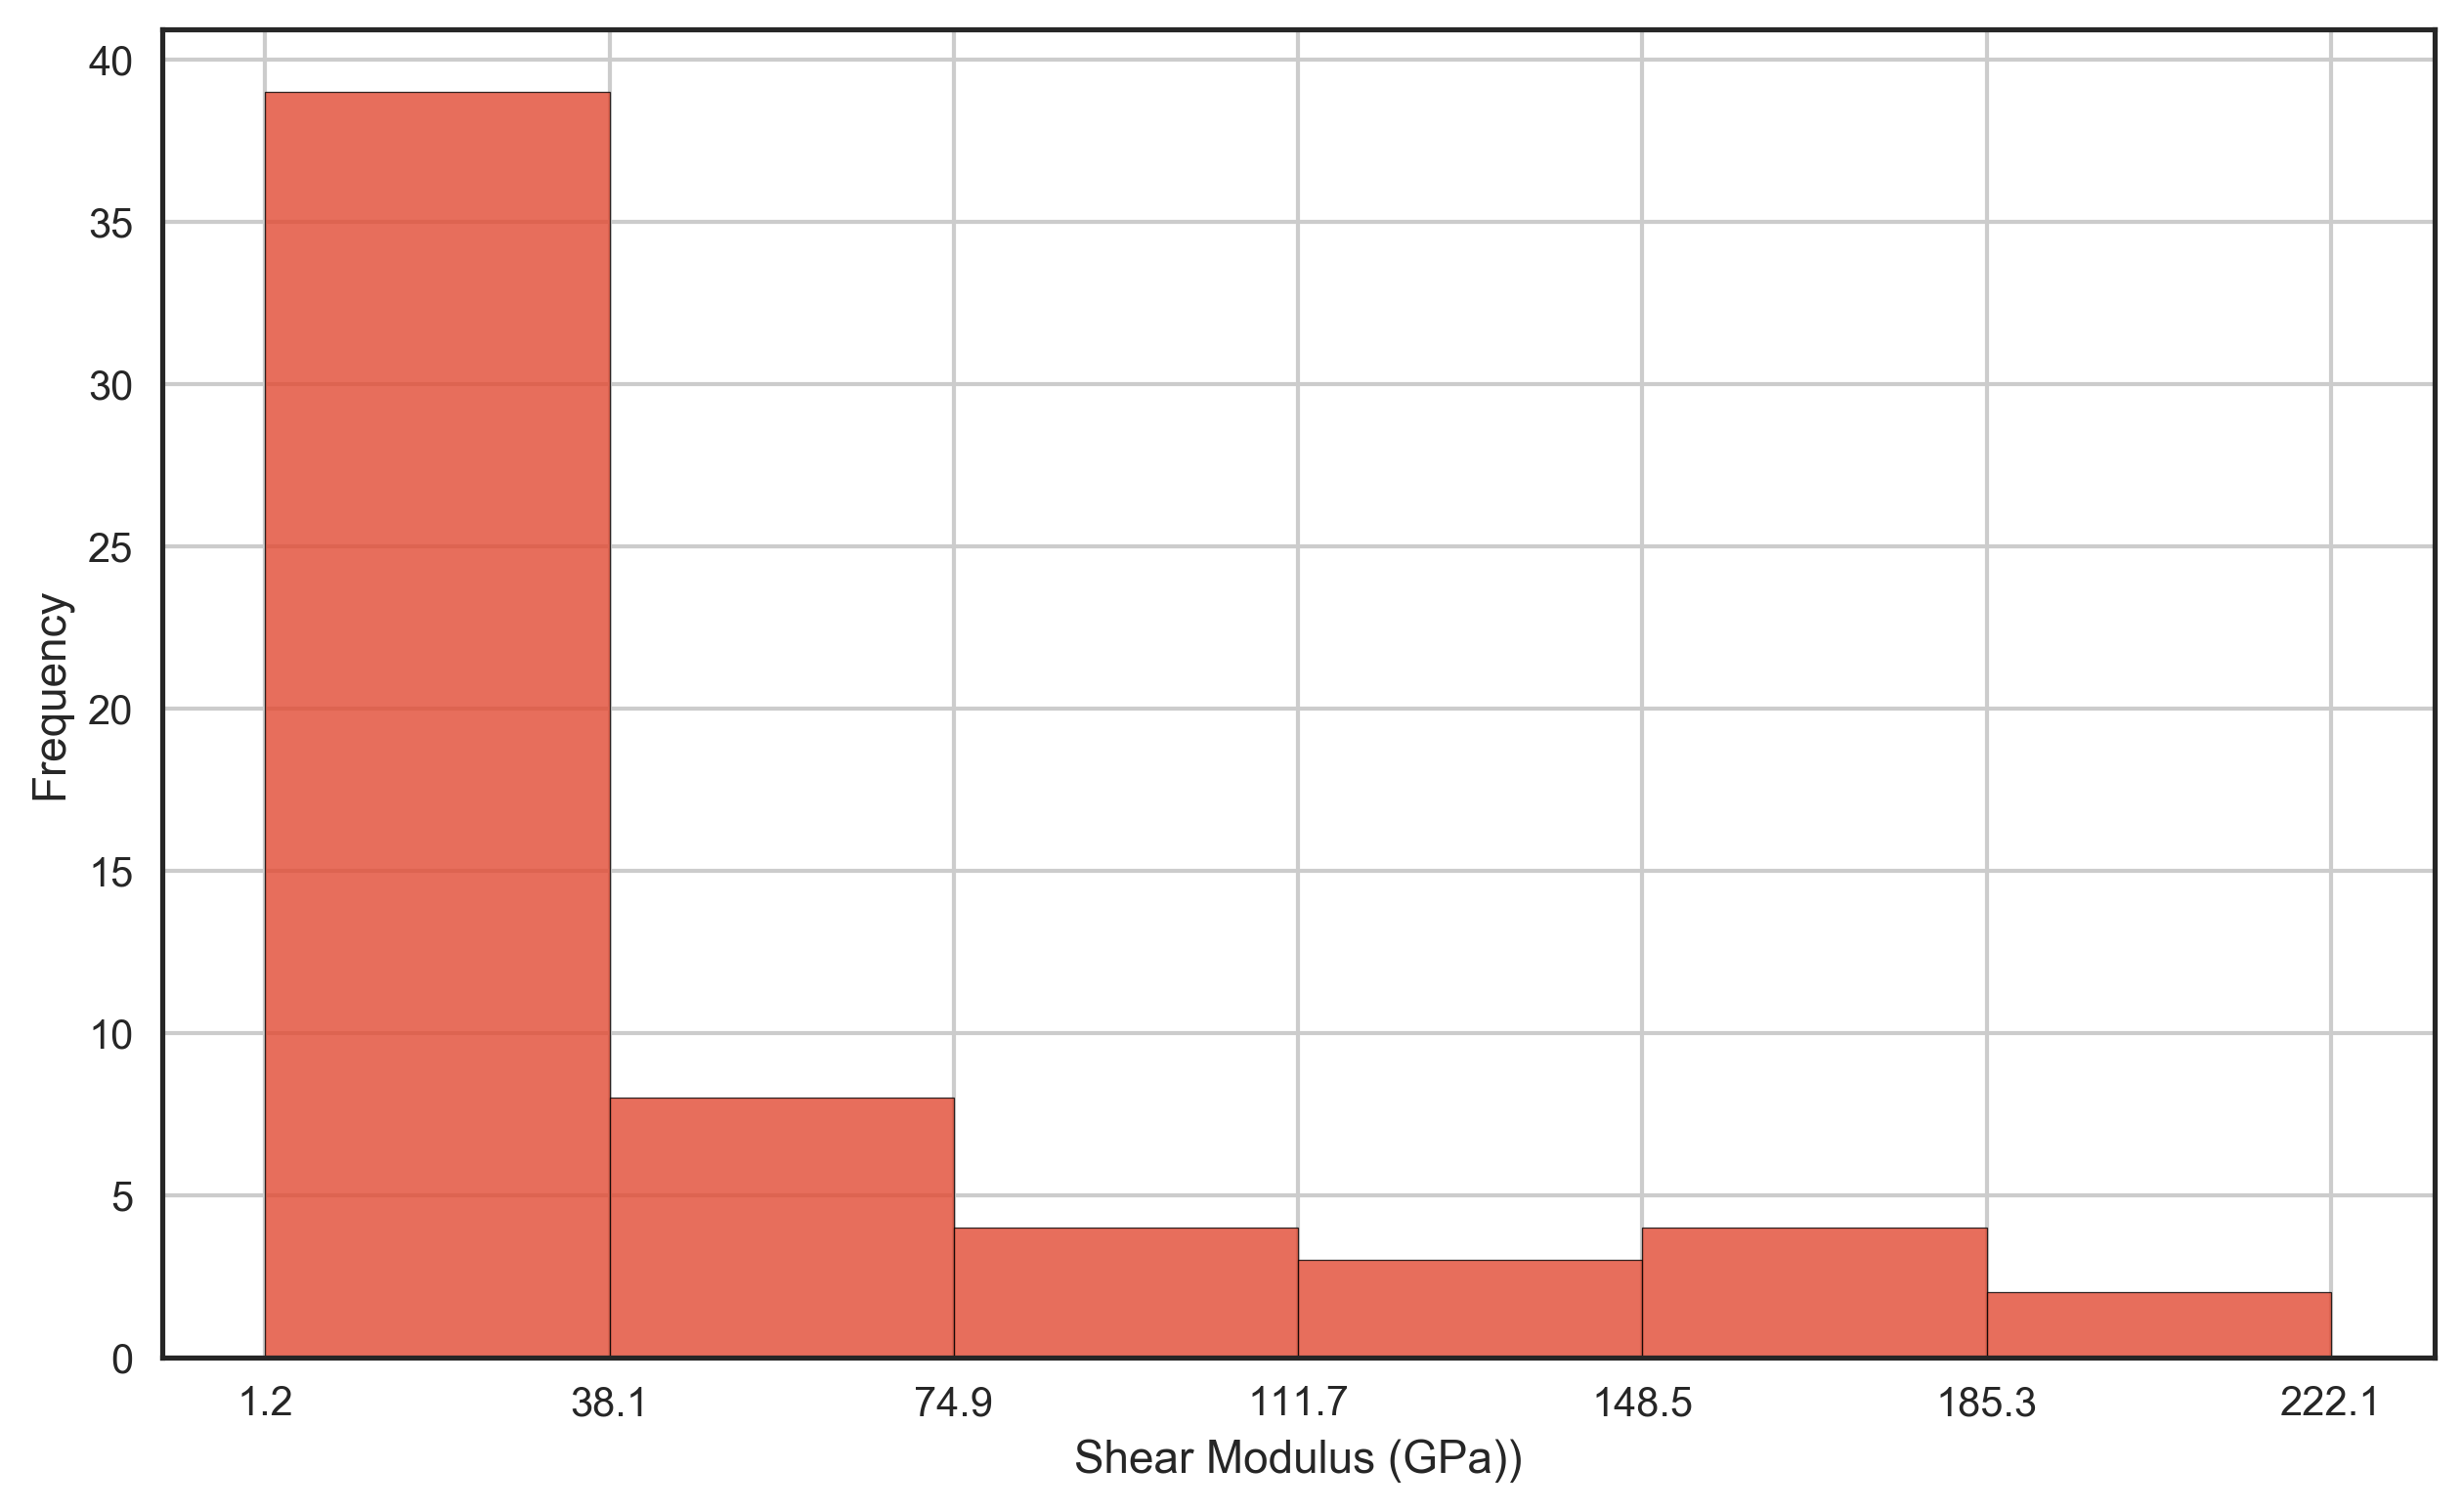
\includegraphics[width=\textwidth*3/4]{assets/elements_histogram.png}
\end{figure}
\begin{figure}
\caption{Frequencies of the Shear Modulus of the Elements in psi \cite{elements}}
\centering
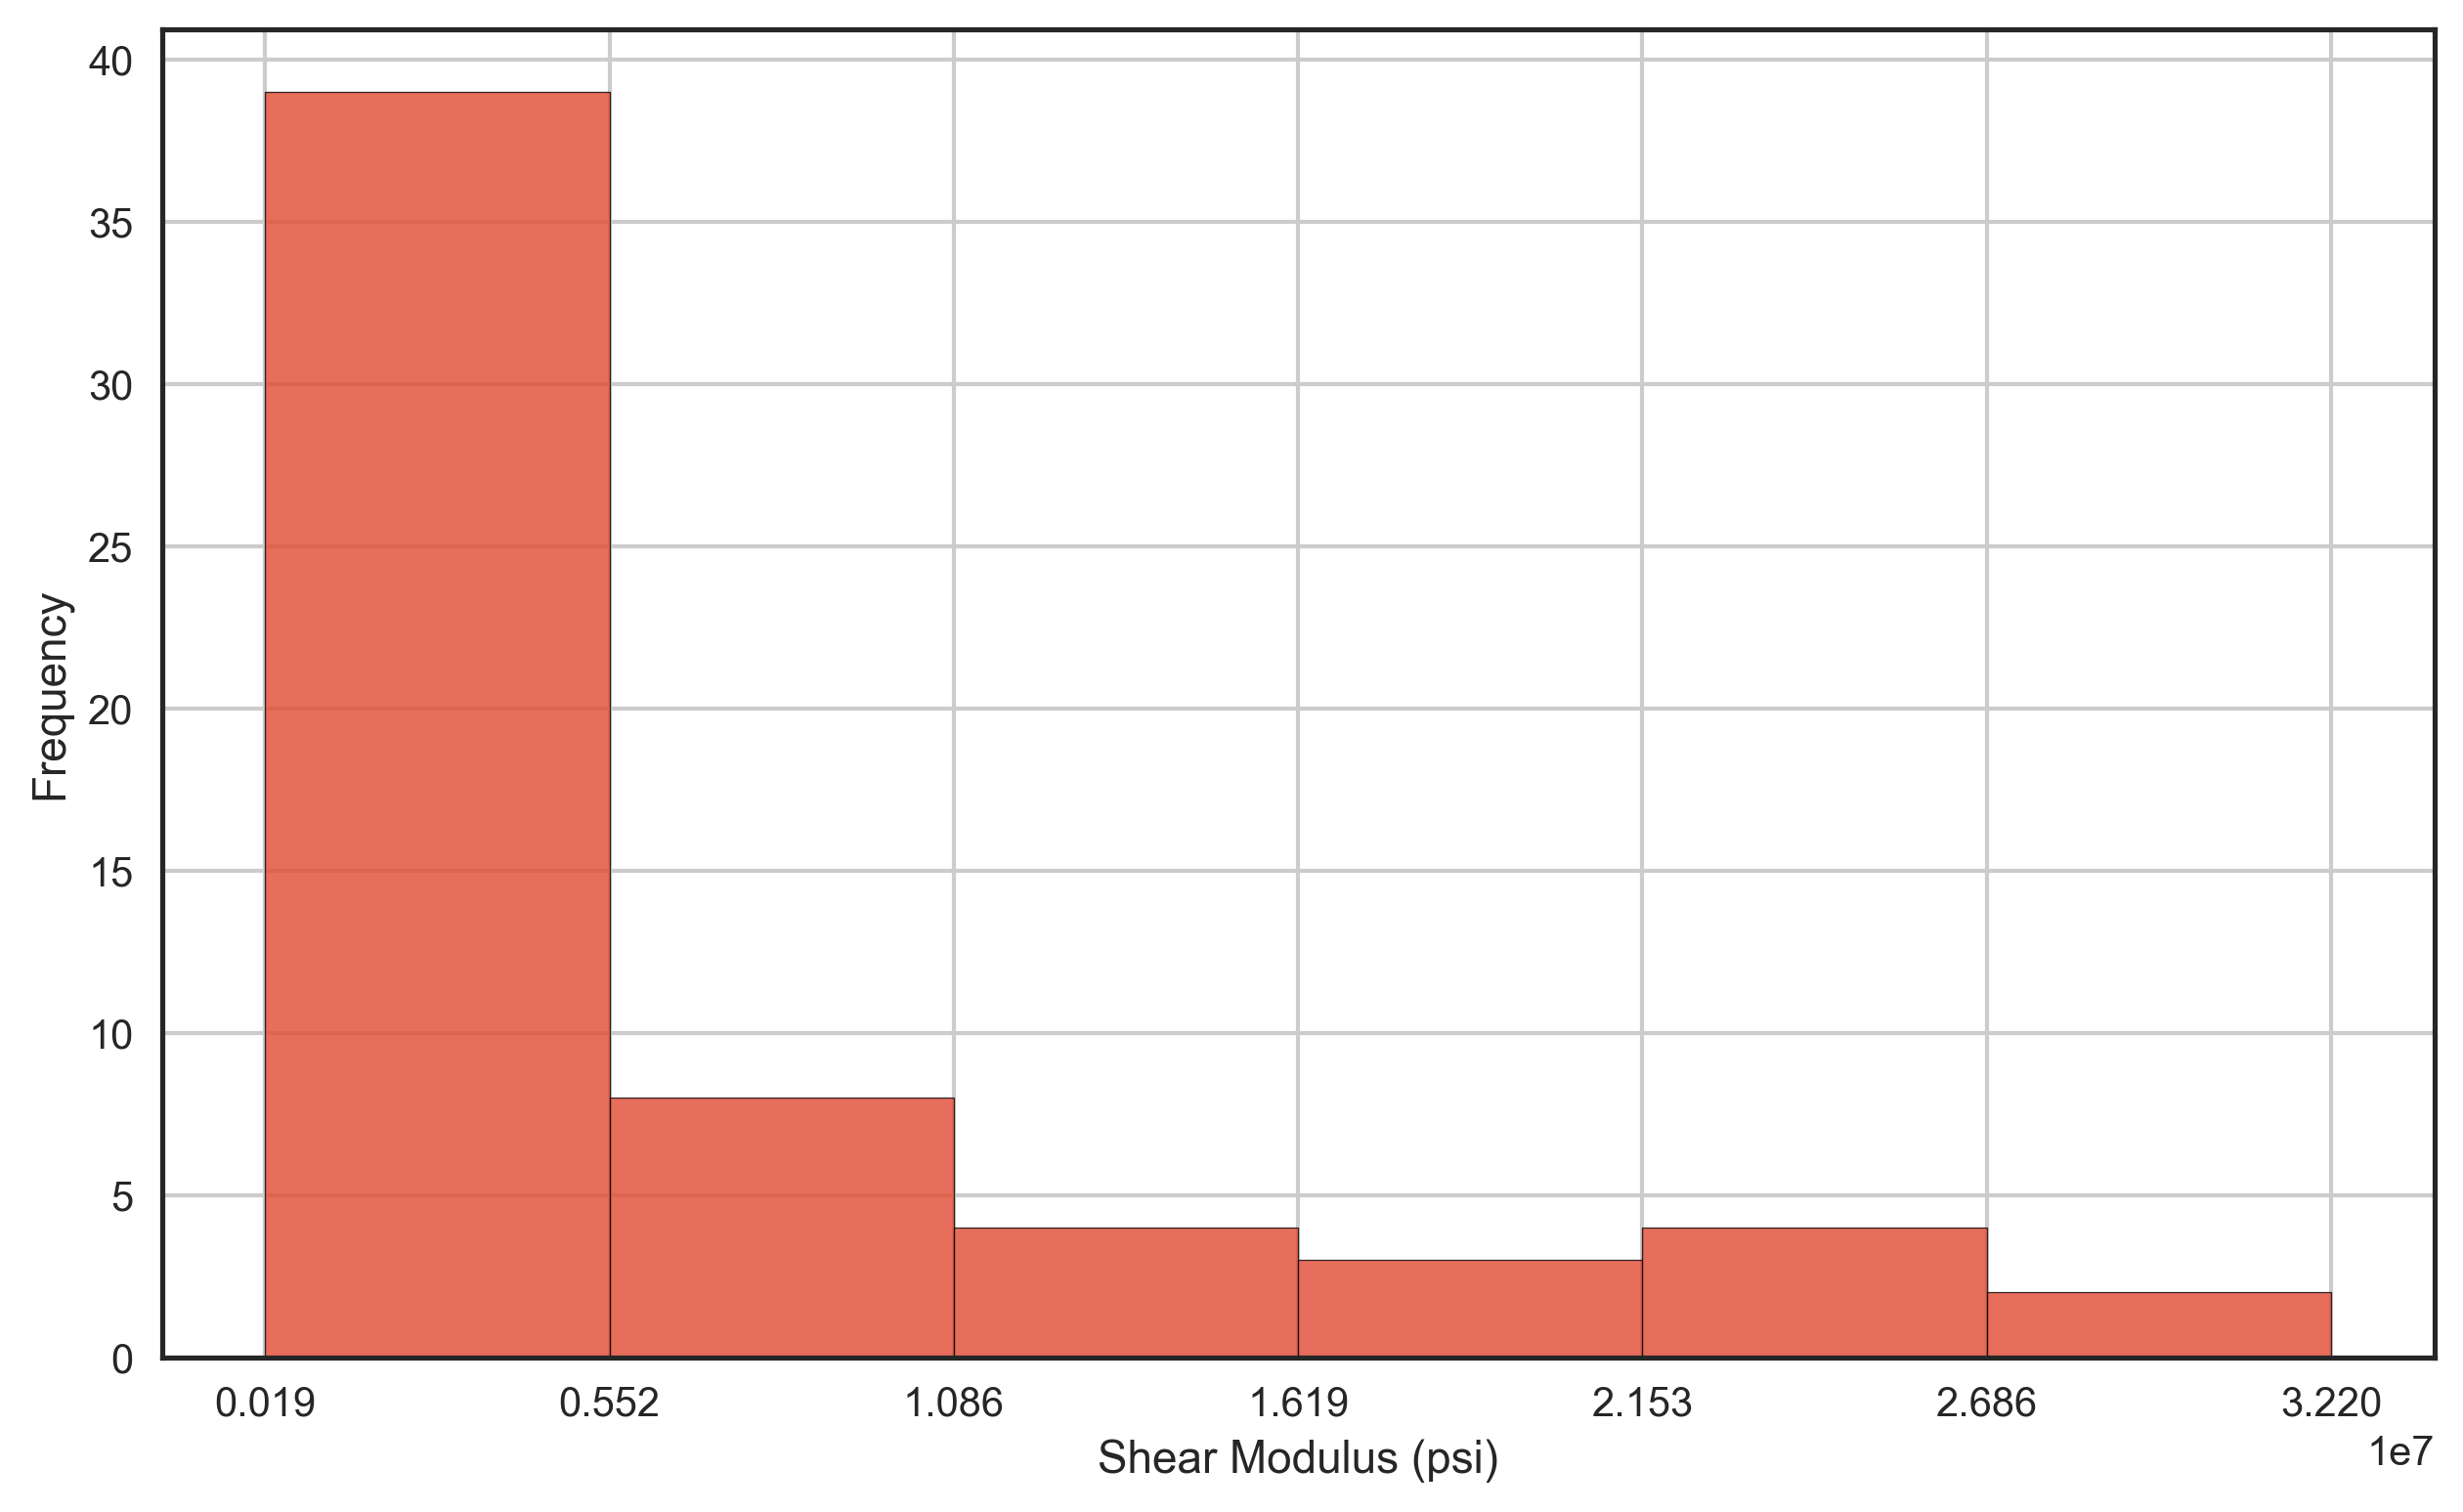
\includegraphics[width=\textwidth*3/4]{assets/elements_histogram_psi.png}
\end{figure}
The Shear Modulus in psi was calculated by multiplying the Shear Modulus in GPa by a factor of 145038, as 1 gigapascal is 145038 pounds per square inch. Interestingly, the histograms look identical, with identical frequencies, since the category length between the bins have been scaled by the same amount. This shows that changing a dataset’s units by a multiplicative factor would not affect the histogram of the frequencies of the data, as long as the bin length is scaled by the same factor.\\
Now, let us see if the leading digits follow Benford's law.  \\\\
\begin{figure}[h]
\caption{Leading digits of the Shear Modulus of the Elements in GPa \cite{elements}}
\centering
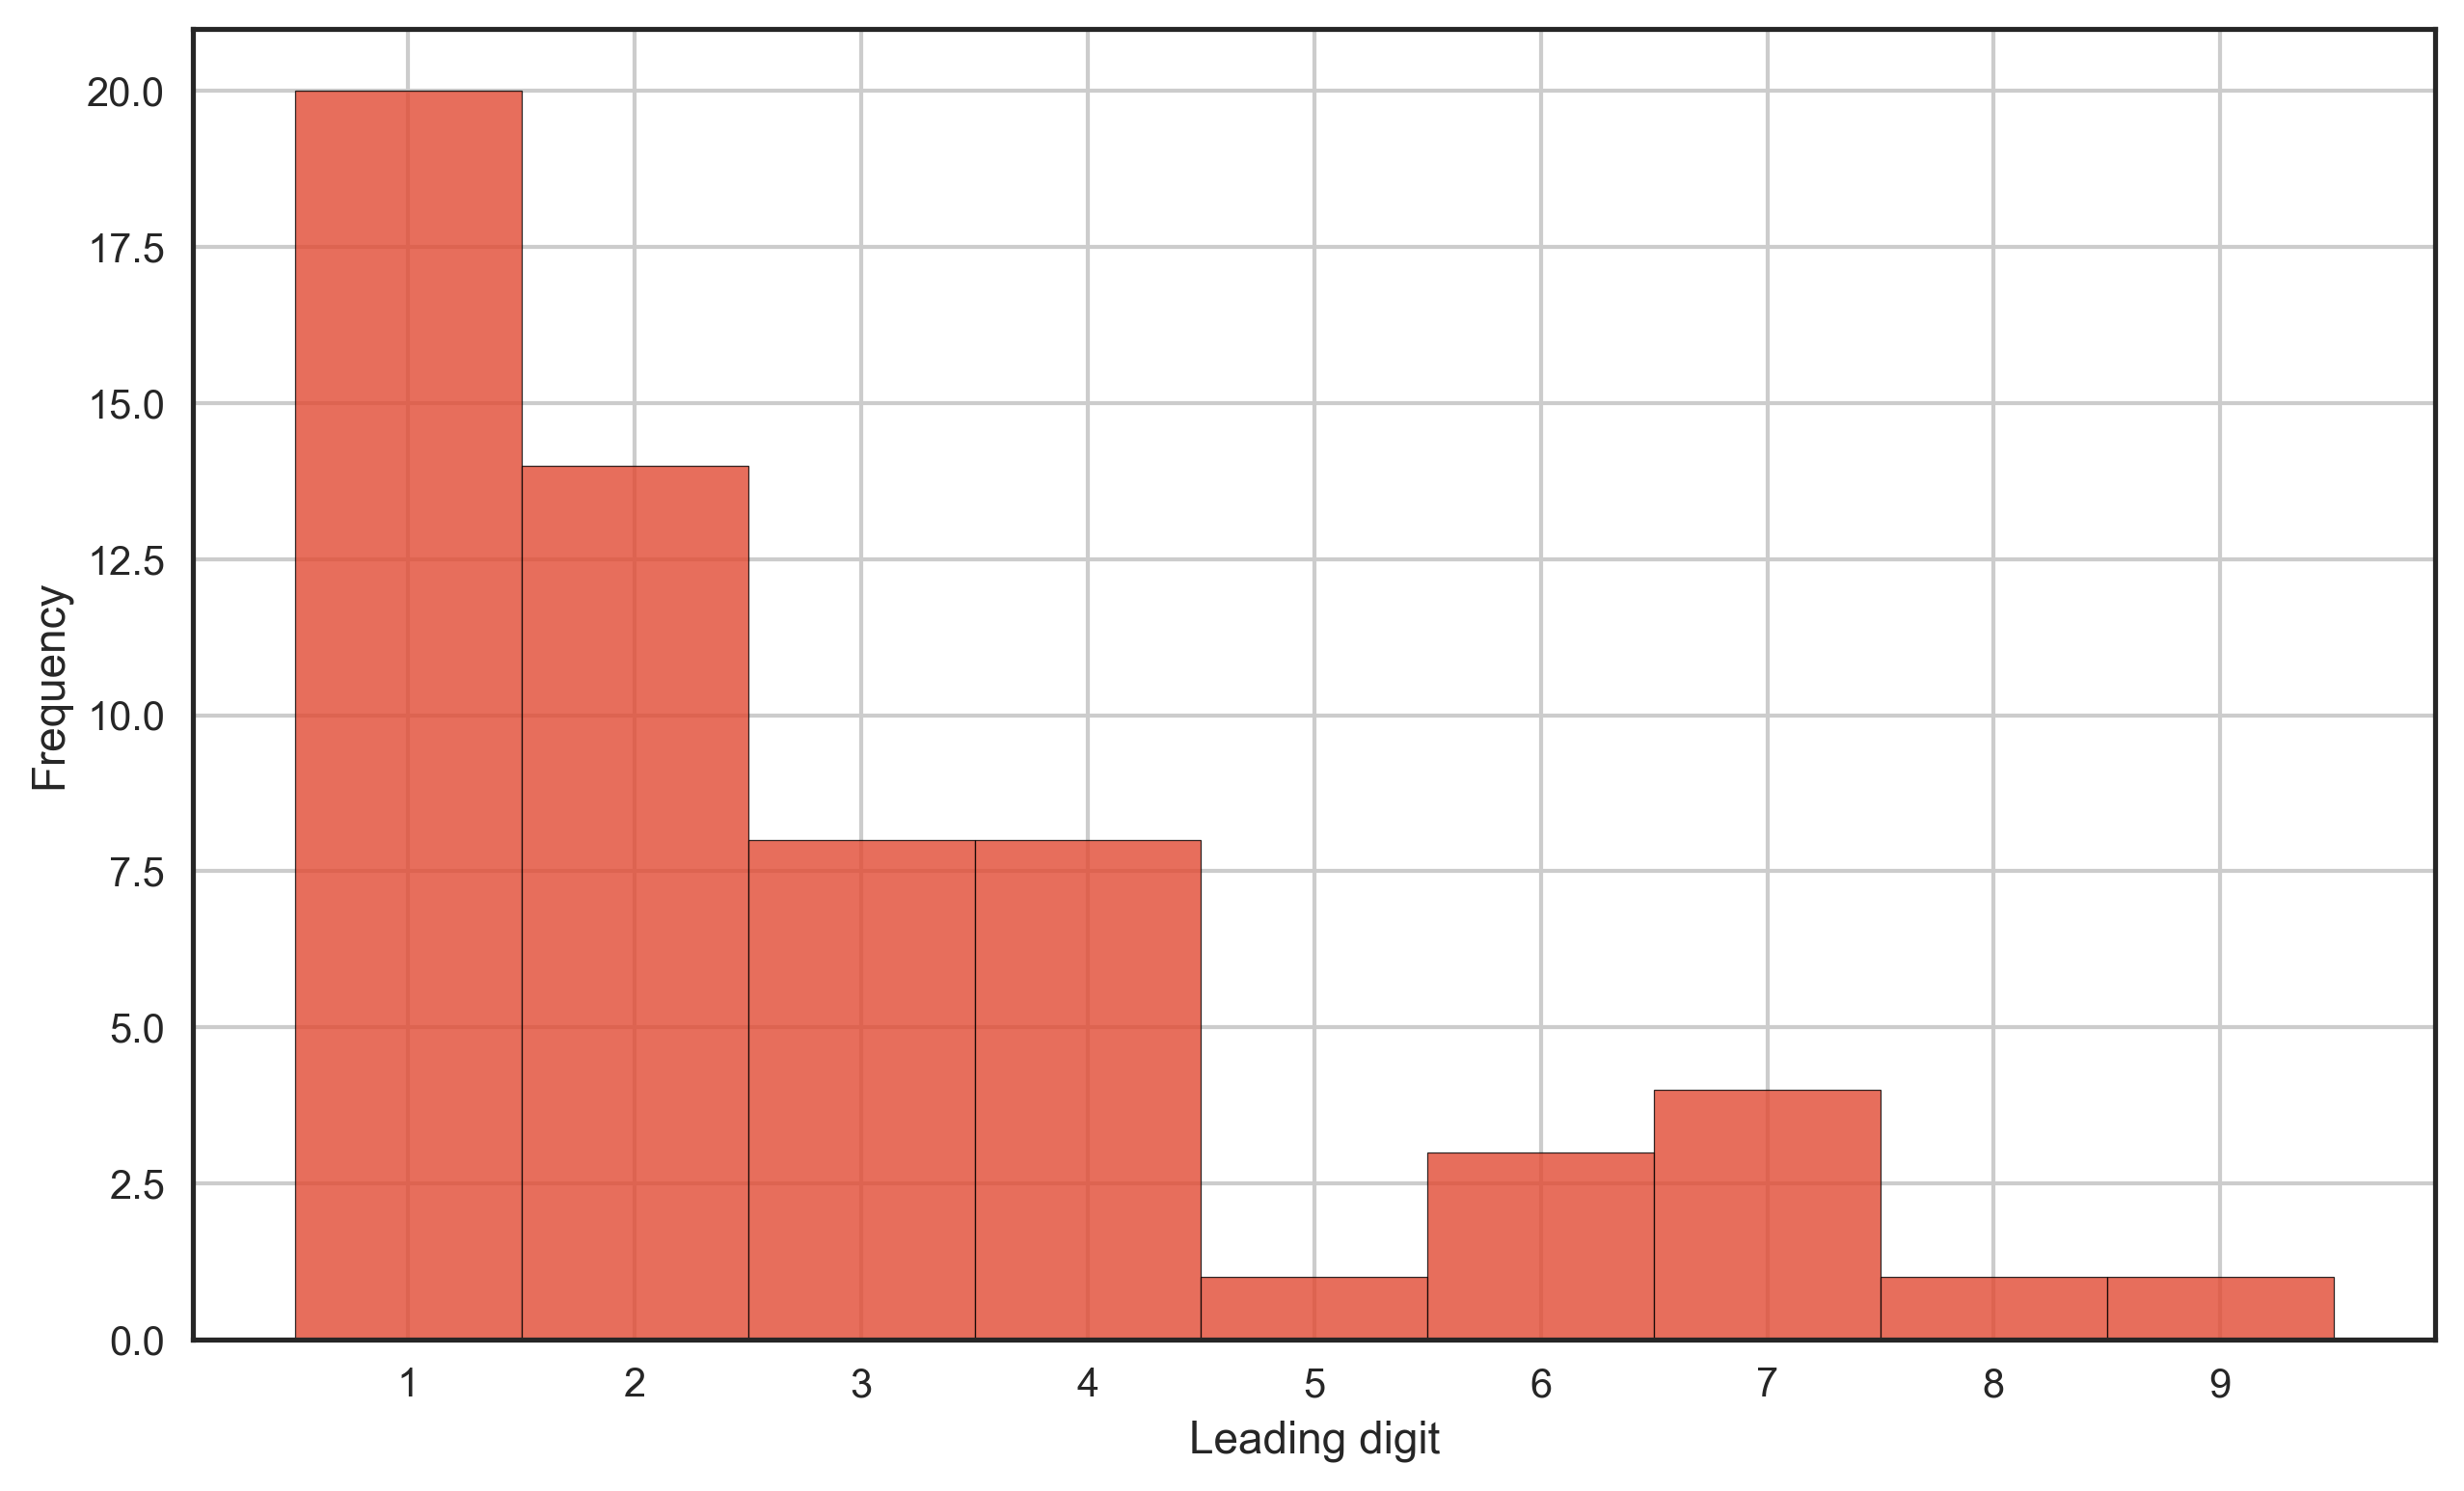
\includegraphics[width=\textwidth*3/4]{assets/digits.png}
\end{figure}
According to Figure 3, it can be seen that 1 is the most common leading digit, 2 is second common, and the frequencies of the remaining digits decrease. Note that these do not follow Benford's distribution perfectly; there are more digits who lead with 6, 7 rather than 5, 8, 9. However, the frequencies are clearly not uniform. \\\\
To see the scale invariance of Benford's law, the leading digits of the scaled values to psi are plotted in Figure 4.
\begin{figure}[h]
\caption{Leading digits of the Shear Modulus of the Elements in psi \cite{elements}}
\centering
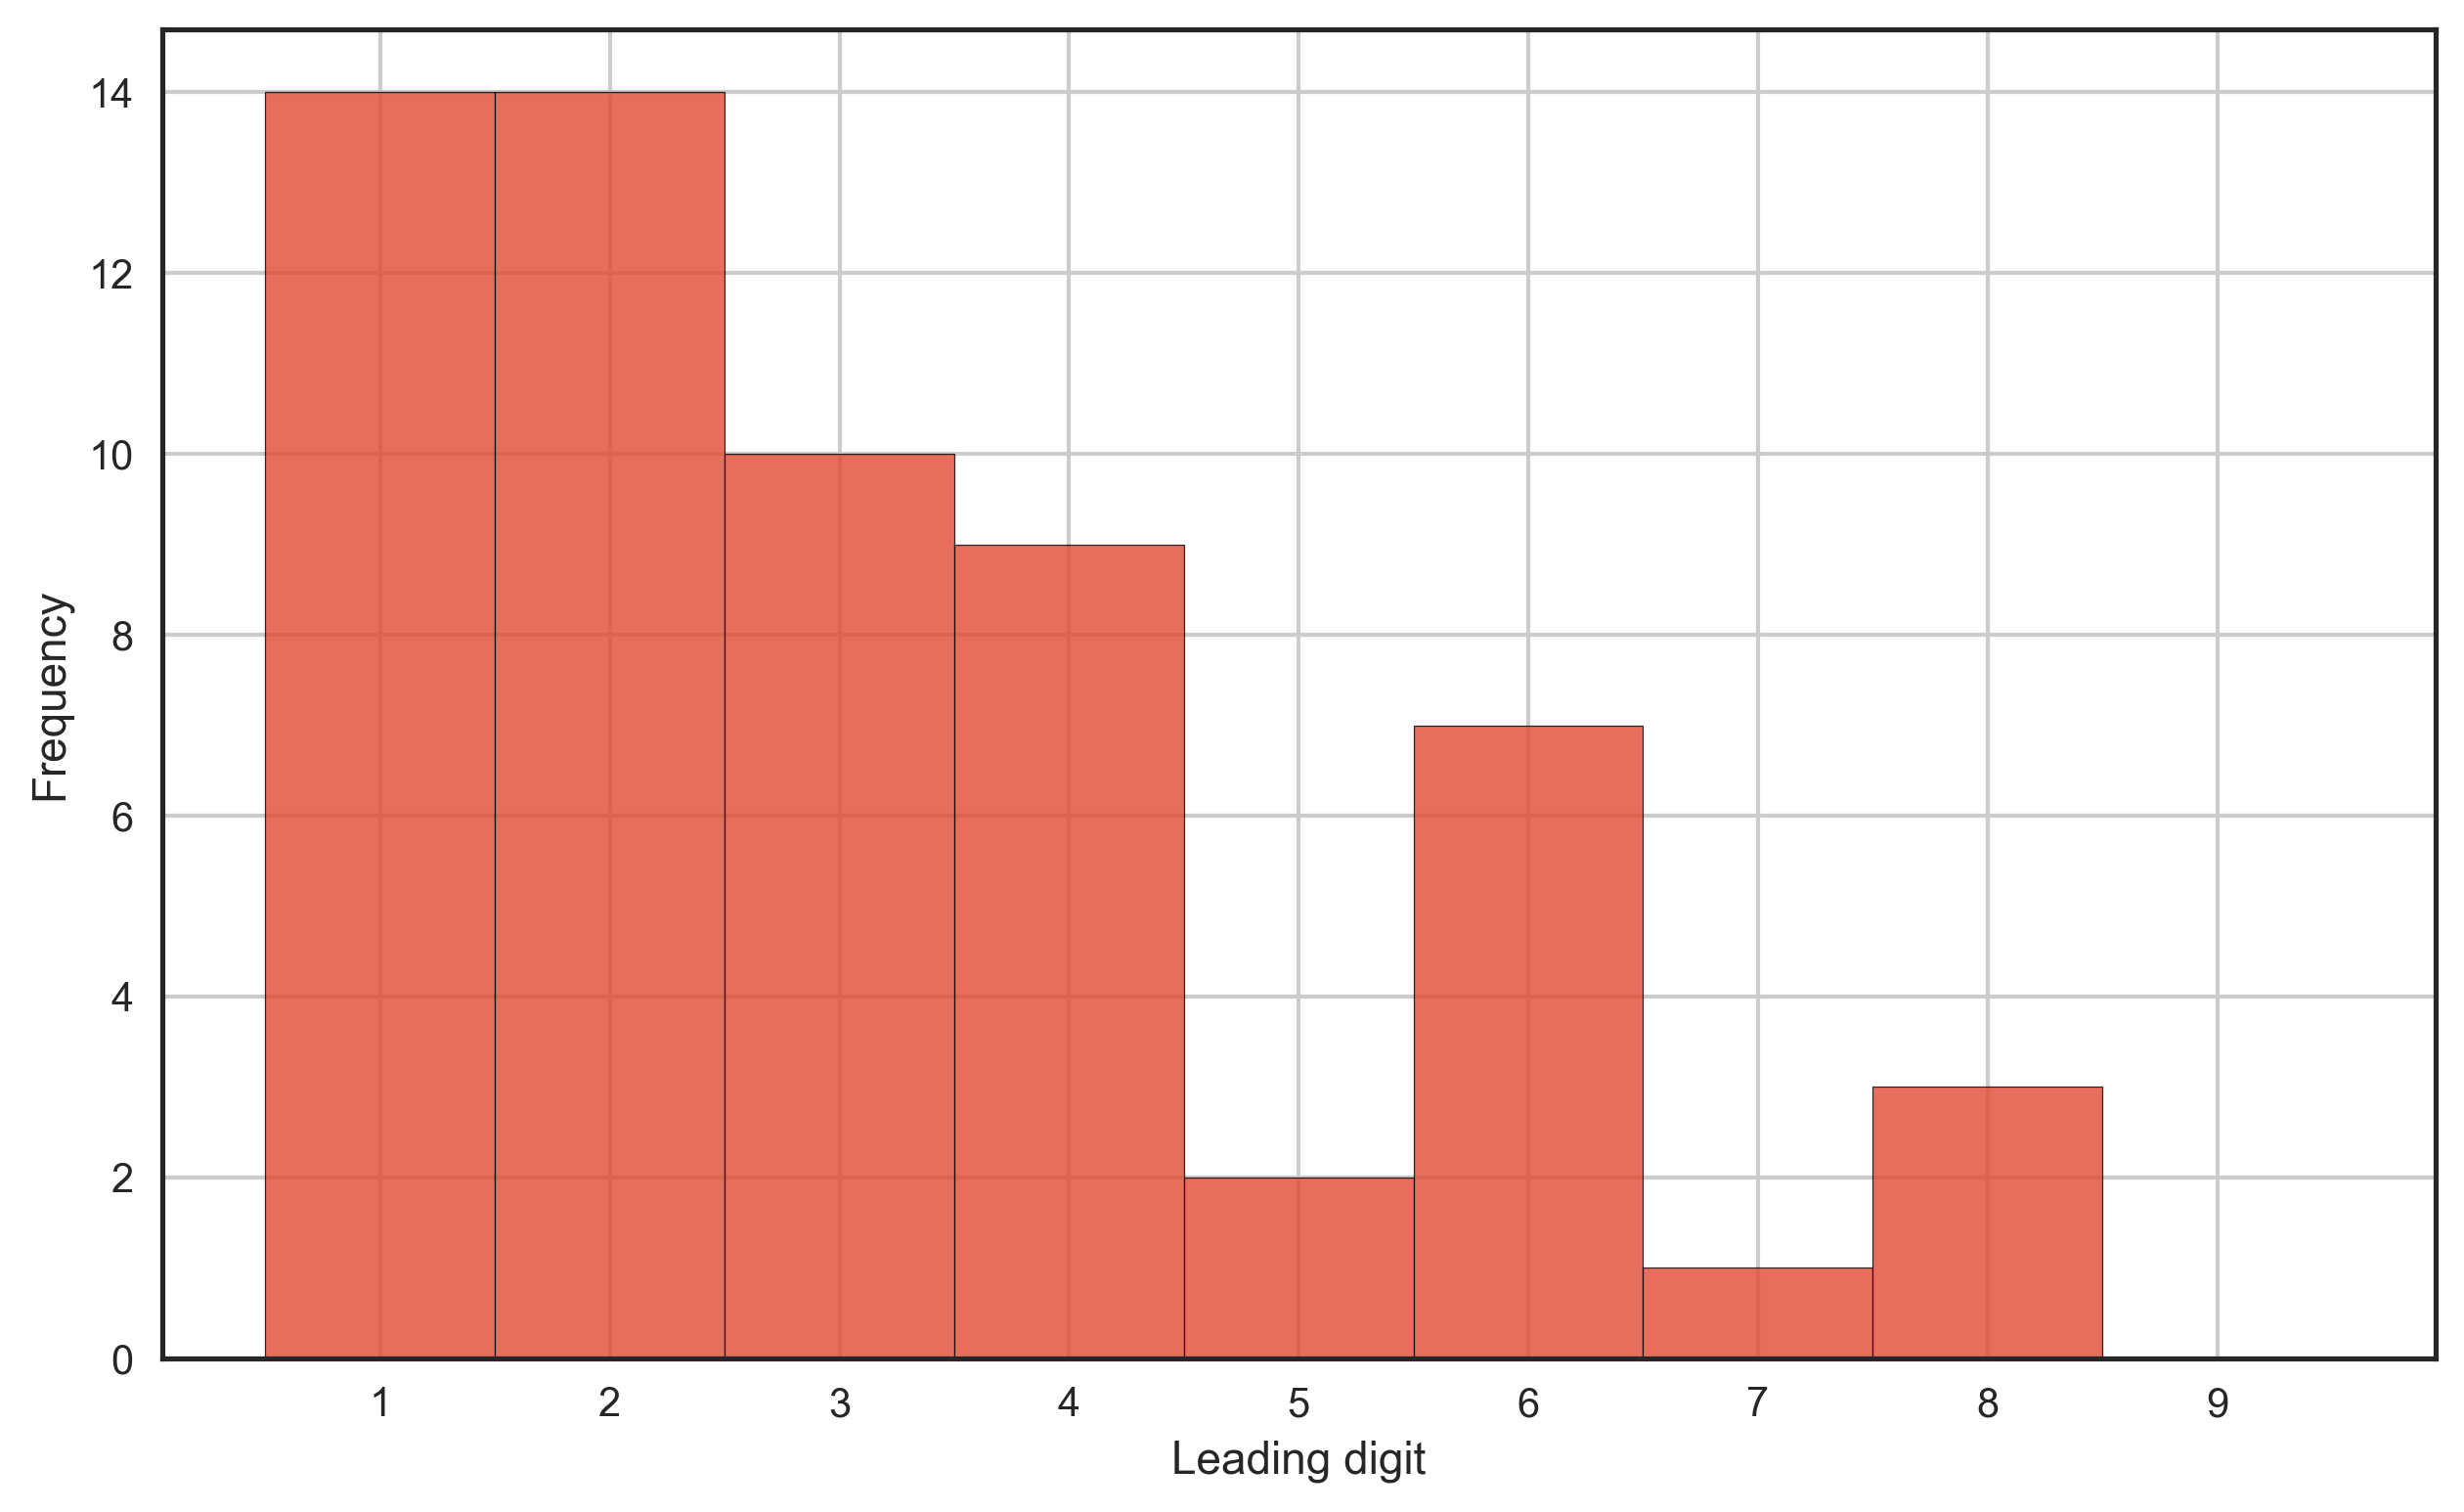
\includegraphics[width=\textwidth*3/4]{assets/digits_psi.png}
\end{figure}
From Figure 4, we can see that there is a similar trend that the leading digits tend to cluster towards the left. Note that this trend is not perfect; it does not mirror the leading digits of the GPa dataset in the same way as the histograms do for the raw frequencies.

\pagebreak
\section{Pinkham's Proof}
Pinkham \cite{pinkham} provides a systematic proof of Benford’s law. For a random set of data without physical constraint, for example the Young’s modulus of a given set of metals, F(x) denotes the ratio of data less than x. For example, F(10) refers to the ratio of the amount of data less than 10 to the total amount of data. Then, the ratio of data with the first leading digit starting from 1 to x-1 is given by:
\begin{equation}
\setcounter{equation}{1}
D(x) = \sum_{m=-\infty}^{\infty} [F(x10^m) - F(10^m)]
\end{equation}

Let us look at this using an example. Suppose x=2, then the summation on the right sums over the ratio of data between 0.1-0.2, 10-20, 100-200, 1000-2000, ..., all of which start with the digit 1. In other words, the summation gives the ratio of data with the first leading digit to be 1. For the same reason, D(3) gives the probability of finding a number starting with 1 or 2, so it is cumulative.\\

Later on, Pinkham introduced the invariance principle, which essentially says that the distribution of leading digits does not depend on the units of measurement. A very straightforward example would be a list of river lengths in a specific country. The ratio of the amount of data with the leading digit 1 is the same whether the units of measurement is in metres or kilometres. If we were to introduce a constant $\alpha$ as the conversion factor, then the invariance principle can be defined by: 

\begin{flalign}
 D(x) & = \sum_{m=-\infty}^{\infty} [F(x10^m) - F(10^m)] \hspace{-5ex} &  x \in \{1, 2, 3, 4, 5, 6, 7, 8, 9 \} \notag\\
& = \sum_{m=-\infty}^{\infty} [F(\frac{x}{\alpha}10^m) - F(\frac{1}{\alpha}10^m)]
\end{flalign}

D(x) is still the ratio of numbers with the leading digits from 1 to x-1. To avoid making it too complicated, let us stick with the river length example. In this case, the conversion factor is $\alpha$ = 1000. X can be any random integer from 2 to 9. Let’s assume X=3. What this equation means is that the ratio of data with leading digits 1 or 2 in the unit of meters is the same as the ratio of data with leading digit 1 or 2 in the unit of kilometers, but the corresponding value in kilometers is 1000 times smaller. Or one can understand the equation in this way: the ratio of river with length 1000-3000 meters long is the same as the ratio of river with length 1km-3km long.

\begin{flalign}
D(\frac{x}{\alpha}) & = \sum_{m=-\infty}^{\infty} [F(\frac{x}{\alpha}10^m) - F(10^m)] & (\alpha > 0)\\
D(\frac{1}{\alpha}) & = \sum_{m=-\infty}^{\infty} [F(\frac{1}{\alpha}10^m) - F(10^m)] & (\alpha > 0)\\
(3) - (4) & = \sum_{m=-\infty}^{\infty} [F(\frac{x}{\alpha}10^m) - F(10^m)] - \sum_{m=-\infty}^{\infty} [F(\frac{1}{\alpha}10^m) - F(10^m)] \notag \\
& = \sum_{m=-\infty}^{\infty} F(\frac{x}{\alpha}10^m) - F(\frac{1}{\alpha}10^m) = D(x)  \notag\\
&\therefore \hspace{1ex} D(\frac{x}{\alpha}) - D(\frac{1}{\alpha}) = D(x) \notag
\end{flalign}

Equation 5 shows that the function D has a similar property with the function $log_{10}(x)$. Therefore, we can deduce that $D(x)=log_{10}(x)$, which tells us that the ratio of data with the leading digit from 1 to x-1 is equal to $log_{10}(x)$. Furthermore, the ratio of data starting with digit x equals to $log(x+1) - log(x)$.

\pagebreak
\section{Benford's Law with Non-leading Digits}

As observed in the previous sections, Benford's distribution models the probability of a digit occurring as the first digit of a sequence in naturally occurring systems. The probability of this distribution \cite{benford} is modelled by \\ 
\begin{equation*}
P = log(n+1)-log(n) 
\end{equation*}


So, the probability of the number 1 being the first digit of a sequence is log(2) - log(1). However, this formula can be extended to other non-leading digits in the sequence. \\
If the probability of a number occurring as the first digit is P = log(n+1)-log(n), then the probability of the first two numbers of the sequence being 10 is log(11) - log(10). Therefore, if we wanted to find the probability that the second digit of a sequence was 0, we would have to add up the probabilities of the cases in which this is possible (10, 20, 30, 40, 50, 60, 70, 80 and 90). So \\
\begin{equation*}
\begin{split}
P(\text{second digit} = 0) & = log(11)-log(10)+log(21)-log(20)+...+log(91)-log(90) \\
& \approx 0.119 = 11.9\%
\end{split}
\end{equation*}

Similarly, the probability that the second digit will be a 1 is 0.114, the second digit being a 2 is 0.109, and so on. This is how we can use Benford's law to predict the second digit. We can already see that the probability that the second digit will be a 0 is greater than the probability the second digit will be a 1, but it can also be seen that while the probabilities of greater numbers occurring is still less, the difference is now significantly lower. This difference continually decreases as we increases the order of decimal places, until we reach the 9th decimal place, when the probability of all number occurring is equal, at 0.1.

\section{Shortcomings of Pinkham's Approach}

Theodore Hill \cite{hill} provided several counter arguments to the common approaches used by several authors to prove Benford's Law. Specifically, these approaches included discrete, continous methods, as well as the hypothesis of scale-invariance which Pinkham's approach focused on. \\
For the discrete methods, proofs have made the assumption that the data set is based on the natural numbers, so some density function mapping to a set of numbers $F_d = \{1, 2, 3, 4, 5, 6, 7, 8, 9\}$ would be natural. Hill shows this to be false - that this set $F_d$ is not in fact a natural density. Further, Benford's data included continous data (such as irrational numbers), which is a significant oversight for a discrete argument. Additionally, for both the discrete and continuous methods, Hill points out that the proofs only prove the finite additivity axiom; that is,
\begin{equation*}
	P\big[\bigcup^N_{n=1}=A_n\big]=\sum^N_{n=1}P\big[A_n\big]
\end{equation*}
They do not, however, satisfy the countable additivity axiom:
\begin{equation*}
	P\big[\bigcup^\infty_{n=1}=A_n\big]=\sum^\infty_{n=1}P\big[A_n\big]
\end{equation*}
thus, it is a weaker proof.\\
The final method is the proof under the assumption that Benford's law would be scale invariant. For something to be scale invariant, it means that for a random variable X, that its distribution is the same as $\alpha X$. The only way for this random variable to be scale invariant is for it to be zero, so that $P[X = 0] = 1$. This is the only random variable that has this property, as \cite{hill_book}
\begin{equation}
	\begin{split}
		P[X \neq 0] & = lim_{a \rightarrow +\infty}P[|X| > a^{-1}] \\
		& = lim_{a \rightarrow +\infty}P[|a^2X| > a] \\
		& = lim_{a \rightarrow +\infty}P[|X| > a] = 0
	\end{split}
\end{equation}
 Thus, since the set $F_d$ does not include zero, the random variable on this density can't be zero, and can't be scale invariant. Additionally, Hill adds that the scale invariance hypothesis has the same problems as the former two methods, so it cannot be strong enough to be a thorough proof.
\pagebreak

\appendix
\section{Appendix}
\subsection{Elastic Properties of the Elements \cite{elements}}

\csvreader[
  longtable=ccccccc,
  table head=
  \toprule \bfseries \thead{Atomic\\Number} &\bfseries \thead{Symbol} & \bfseries \thead{Name} & \bfseries \thead{Shear\\Modulus\\(GPa)} & \bfseries \thead{Shear\\Modulus\\(psi)} & \bfseries \thead{Leading\\Digit\\(GPa)}& \bfseries \thead{Leading\\Digit\\(psi)}\\\midrule\endhead\bottomrule\endfoot,
  late after line=\\,
  before reading={\catcode`\#=12},after reading={\catcode`\#=6}
]{assets/element_data.csv}{1=\one,2=\two, 3=\three, 4=\four, 5=\five, 6=\six, 7=\seven}{\one & \two & \three & \four & \five & \six & \seven}

\pagebreak

\begin{thebibliography}{9}
\raggedright
\bibitem{benford} 
Frank Benford. The law of anomalous numbers. Proc. Amer. Philosophical Soc., 78:551–572, 1938. \texttt{http://www.jstor.org/stable/984802.}
 
\bibitem{hill} 
Theodore P. Hill Base-invariance implies Benford’s law. Proc. Amer. Math. Soc., 123:887–895, 1995.
\texttt{http://www.ams.org/journals/proc/1995-123-03/S0002-9939-1995-1233974-8/.}
 
\bibitem{pinkham} 
Roger S. Pinkham. On the distribution of first significant digits. Ann. Math. Statist., \texttt{32(4):1223–1230, 12}

\bibitem{elements}
Wikipedia. Elastic properties of the elements \text{(data page)} wikipedia, the free encyclopedia, 2013. \url{https://en.wikipedia.org/w/index.php?title=Elastic_properties_of_the_elements_(data_page)} Web. Accessed June 29th, 2015.

\bibitem{hill_book}
Berger, Arno, and Theodore P. Hill. An Introduction to Benford's Law. PRINCETON; OXFORD, Princeton University Press, 2015. JSTOR, \url{www.jstor.org/stable/j.ctt1dr35m0.}

\end{thebibliography}




\bibliography{References}

\end{document}
